\section{First campaign: experiments 1--5}
\label{sec:experiments}
\label{sec:plan}

The experiments are not a chronology. Before training anything, the observations of
Section~\ref{sec:framing} were turned into an ordered list of hypotheses, each changing
exactly one thing and each falsifiable by a single number: (1) a plain encoder--decoder
already finds the main filaments; (2) with fewer than 500 observations the encoder is
the bottleneck, so ImageNet features should beat random initialisation; (3) Dice is
blind to fragmentation, so a topology-aware loss should raise PQ; (4) part of the
residual is the H-alpha \emph{domain} rather than the loss; (5) what limits PQ is
\emph{scale}. Hypotheses 3 and 5 make opposite predictions about where the error
lives, and only one survives contact with the data.

\textbf{Experiments 1--2, baseline and transfer learning.} The from-scratch U-Net
reaches Dice $0.6415$ at the last epoch, still underfitted, with its best threshold at
the edge of the grid -- a sign of poorly calibrated probabilities that points at the
encoder. Replacing it with the pre-trained ResNet18 lifts Dice to $0.6552$ at epoch~8
and, more usefully, flattens the threshold--Dice curve: for a submission whose
threshold must be frozen blind, that calibration is worth more than the point of Dice.

\textbf{Error analysis.} At $0.655$ Dice is already at inter-annotator level, yet PQ is
$0.2505$. Decomposing it: $\mathrm{SQ}=0.61$ (matched instances overlap fine) but
$\mathrm{RQ}=0.38$. The false positives are a swarm of tiny spurious components (median
7~pixels), not fragmentation -- $74\%$ of ground-truth filaments over 32~pixels are
predicted as a single component. This diagnosis is what makes Experiment~3 worth
running, and what post-processing later exploits.

\textbf{Experiment 3, a topology-aware loss -- falsified.} Replacing half of the loss
with Tversky ($\beta = 0.7$) plus clDice (a Dice between soft skeletons) collapses
validation Dice to $0.4937$ and PQ to $0.0618$, while the training loss decreases: the
model optimises the wrong thing successfully. Two lessons. Tversky's recall bias
thickens everything and destroys the calibration transfer learning had bought; and at
$512^2$ many filaments are one or two pixels wide, so the soft skeleton is noise on
exactly the structures clDice was meant to protect -- a scale problem wearing the
costume of a loss problem, and the first hint that hypothesis 5 aims at the right
variable.

\textbf{Experiment 4, the H-alpha domain.} ImageNet normalisation (folded into the
stem), photometric jitter and cosine annealing: Dice $0.6591$, PQ $0.2656$, and the
validation curve now improves to the last epoch instead of stalling at~8.

\textbf{Experiment 5, resolution -- the largest single gain.} Nothing changes except
the input size, $512 \to 1024$. Dice gains one point ($0.6701$) while PQ jumps from
$0.2656$ to $0.3397$, $+28\%$ relative (Figure~\ref{fig:experiment-5}). The asymmetry
is the point: doubling the resolution barely changes how much of the disk is covered
correctly, and changes a great deal about how many filaments exist as recognisable
objects. What looked like a loss problem was a sampling problem.

\begin{table}[ht]
    \centering
    \caption{First campaign. Dice and PQ at threshold $0.5$ without post-processing,
    so the columns are directly comparable; the operating point is selected afterwards
    (Section~\ref{sec:operating}).}
    \label{tab:experiments}
    \small\begin{tabular}{clrrr}
        \toprule
        Exp. & Hypothesis under test & Dice & PQ & Best epoch \\
        \midrule
        1 & U-Net from scratch (baseline)              & 0.6415 & --     & 20 \\
        2 & ImageNet ResNet18 encoder                  & 0.6552 & 0.2505 &  8 \\
        3 & Tversky + clDice loss                      & 0.4937 & 0.0618 & 13 \\
        4 & Photometric aug.\ + normalisation + cosine & 0.6591 & 0.2656 & 18 \\
        5 & Resolution $512 \rightarrow 1024$          & \textbf{0.6701} & \textbf{0.3397} & 15 \\
        \midrule
        \multicolumn{2}{l}{\emph{inter-annotator agreement}} & \emph{0.62} & -- & \\
        \bottomrule
    \end{tabular}
\end{table}

\begin{figure}[ht]
    \centering
    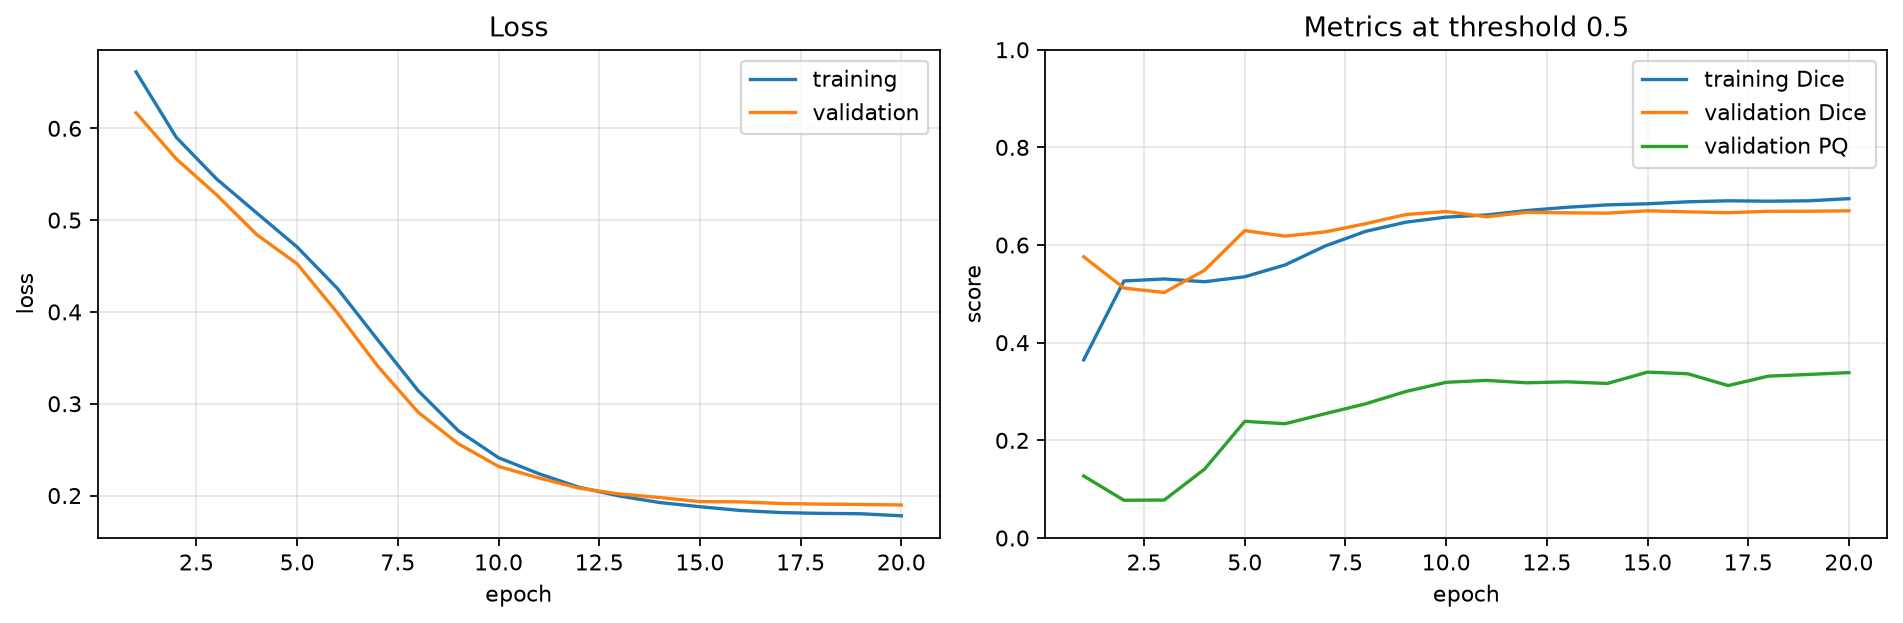
\includegraphics[width=0.72\linewidth]{../experiments/05/plots/training_curves.png}
    \caption{Experiment 5 at $1024 \times 1024$. Validation PQ, the lowest curve on
    the right, gains far more from the change of scale than Dice does.}
    \label{fig:experiment-5}
\end{figure}
